% !TEX program = xelatex
\documentclass[12pt, a4paper]{article}

%% ── 패키지 ──────────────────────────────────────────────────
\usepackage{kotex}                      % 한글 (XeLaTeX / LuaLaTeX)
\usepackage{amsmath, amssymb}
\usepackage{graphicx}
\usepackage{booktabs}
\usepackage{geometry}
\usepackage{caption}
\usepackage{listings}
\usepackage{xcolor}
\usepackage{hyperref}
\usepackage{setspace}
\usepackage{float}

\geometry{left=25mm, right=25mm, top=30mm, bottom=30mm}
\onehalfspacing

%% ── 코드 스타일 ─────────────────────────────────────────────
\lstset{
  language=Matlab,
  basicstyle=\ttfamily\small,
  keywordstyle=\color{blue}\bfseries,
  commentstyle=\color{gray},
  stringstyle=\color{orange!80!black},
  numbers=left,
  numberstyle=\tiny\color{gray},
  frame=single,
  breaklines=true,
  captionpos=b,
  tabsize=4,
}

%% ── 제목 정보 ───────────────────────────────────────────────
\title{\Large 진동학 Homework \#2}
\author{
  전북대학교 산업정보시스템공학과 \\
  202116971 \; 김영환
}
\date{}

%% ════════════════════════════════════════════════════════════
\begin{document}

\maketitle
\tableofcontents
\newpage

%% ────────────────────────────────────────────────────────────
\section{해석 조건}

공통으로 사용한 파라미터는 표~\ref{tab:params}와 같다.

\begin{table}[H]
\centering
\caption{공통 파라미터}
\label{tab:params}
\begin{tabular}{lll}
\toprule
항목 & 기호 & 값 \\
\midrule
가진력 진폭       & $F$      & 10 N \\
바닥 변위 진폭    & $Y$      & 0.01 m \\
주파수 범위       & $\omega$ & 0.1 -- 160 rad/s \\
기준 질량         & $m$      & 5 kg \\
기준 감쇠         & $c$      & 50 N$\cdot$s/m \\
기준 강성         & $k$      & 5000 N/m \\
\bottomrule
\end{tabular}
\end{table}

변화 범위는 공진점이 탐색 범위 안에 들어오고, 저감쇠부터 고감쇠까지 차이가 충분히 드러나도록 설정하였다.

%% ────────────────────────────────────────────────────────────
\section{문제 1. 조화 외력 가진 (Harmonic Force Excitation)}

\subsection{이론}

운동방정식은

\begin{equation}
  m\ddot{x} + c\dot{x} + kx = F\sin(\omega t)
\end{equation}

정상상태 변위 진폭은

\begin{equation}
  X = \frac{F}{\sqrt{(k - m\omega^2)^2 + (c\omega)^2}}
  \label{eq:p1}
\end{equation}

\subsection{(a) 질량 $m$ 변화}

$c = 50$ N$\cdot$s/m, $k = 5000$ N/m 고정.

\begin{figure}[H]
\centering
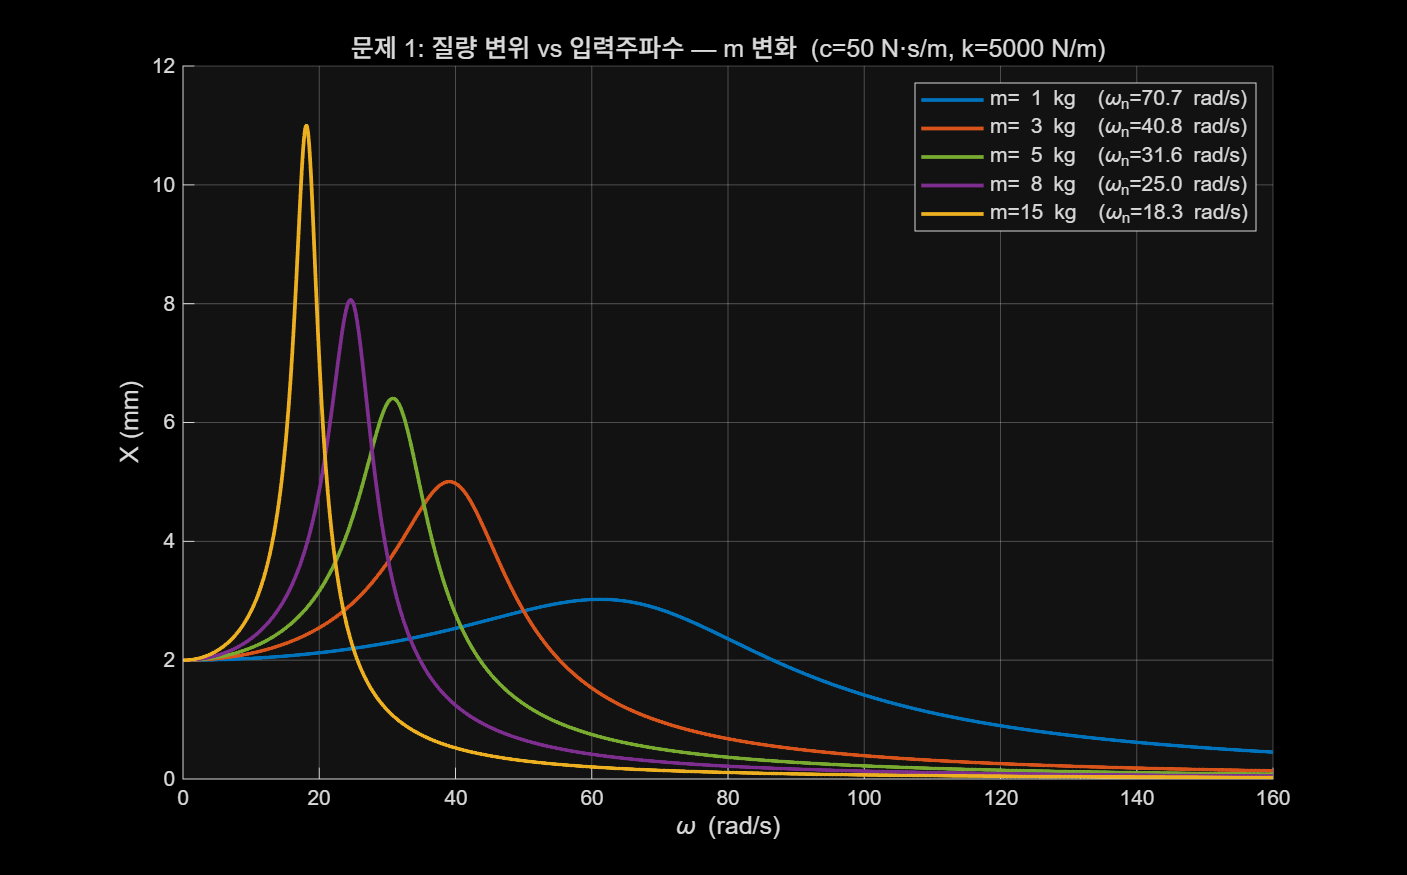
\includegraphics[width=0.80\linewidth]{figures/p1_vary_m.png}
\caption{질량 변위 vs 입력주파수 — $m$ 변화 ($c=50$, $k=5000$)}
\label{fig:p1m}
\end{figure}

\begin{table}[H]
\centering
\caption{$m$ 변화에 따른 고유진동수 및 최대 변위}
\label{tab:p1m}
\begin{tabular}{rrr}
\toprule
$m$ (kg) & $\omega_n$ (rad/s) & $X_{\max}$ (mm) \\
\midrule
1  & 70.7 & 3.02  \\
3  & 40.8 & 5.00  \\
5  & 31.6 & 6.41  \\
8  & 25.0 & 8.06  \\
15 & 18.3 & 11.00 \\
\bottomrule
\end{tabular}
\end{table}

\begin{itemize}
  \item $m$이 커질수록 $\omega_n = \sqrt{k/m}$이 작아져 공진점이 저주파 쪽으로 이동하였다.
  \item 공진 부근 최대 변위는 3.02 mm에서 11.00 mm로 증가하였다.
  \item 고주파에서는 $X \approx F/(m\omega^2)$이므로 큰 질량일수록 응답이 더 빨리 감소하였다.
\end{itemize}

\subsection{(b) 감쇠 $c$ 변화}

$m = 5$ kg, $k = 5000$ N/m 고정.

\begin{figure}[H]
\centering
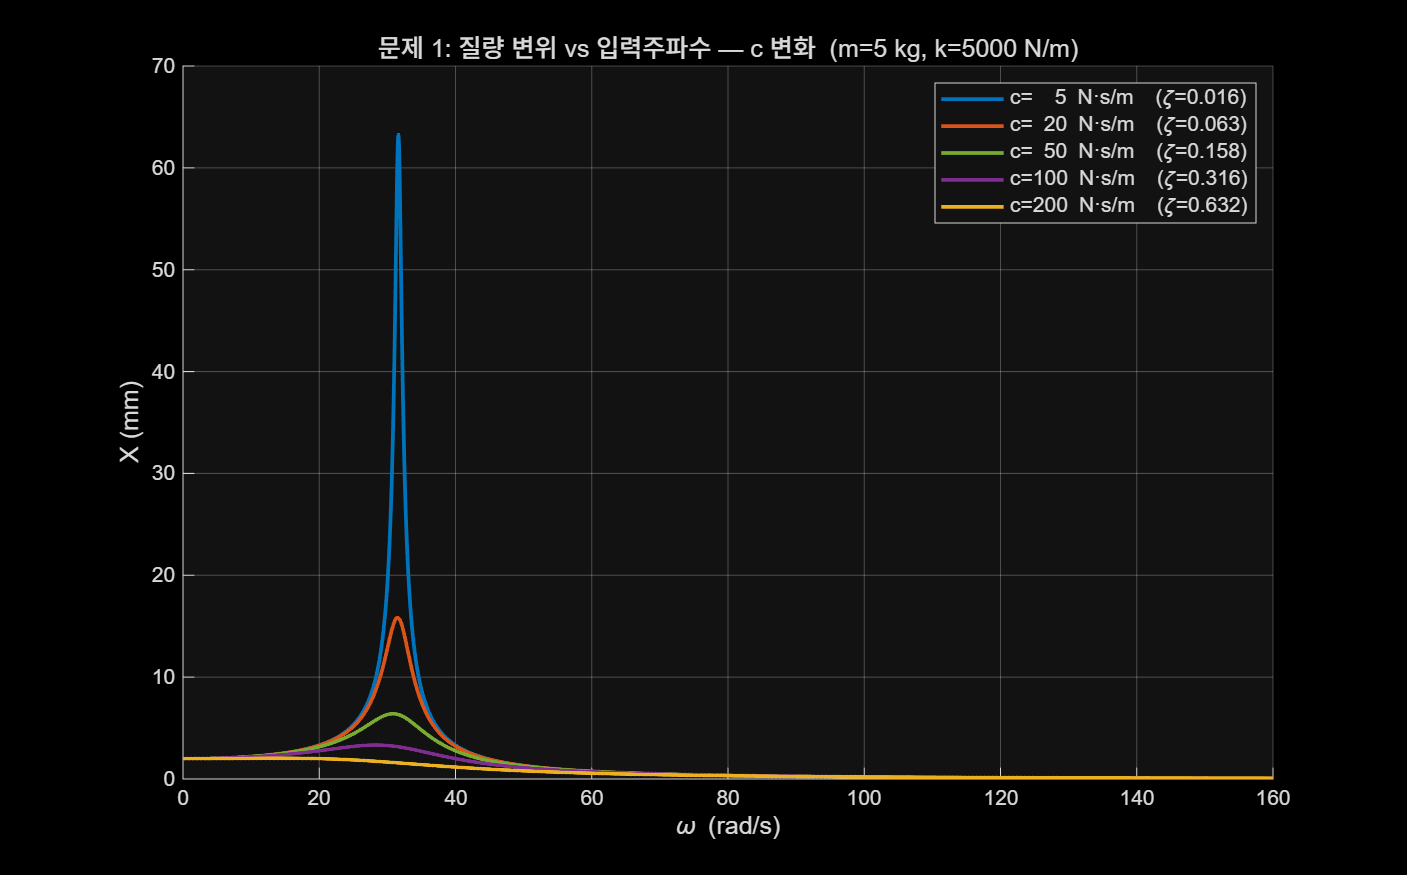
\includegraphics[width=0.80\linewidth]{figures/p1_vary_c.png}
\caption{질량 변위 vs 입력주파수 — $c$ 변화 ($m=5$, $k=5000$)}
\label{fig:p1c}
\end{figure}

\begin{table}[H]
\centering
\caption{$c$ 변화에 따른 감쇠비 및 최대 변위}
\label{tab:p1c}
\begin{tabular}{rrr}
\toprule
$c$ (N$\cdot$s/m) & $\zeta$ & $X_{\max}$ (mm) \\
\midrule
5   & 0.016 & 63.25 \\
20  & 0.063 & 15.84 \\
50  & 0.158 &  6.41 \\
100 & 0.316 &  3.33 \\
200 & 0.632 &  2.04 \\
\bottomrule
\end{tabular}
\end{table}

\begin{itemize}
  \item 감쇠는 자연주파수 자체를 거의 바꾸지 않아 피크 위치는 유사하게 유지되었다.
  \item 공진 피크 크기는 $c=5$일 때 63.25 mm에서 $c=200$일 때 2.04 mm로 크게 감소하였다.
  \item 감쇠는 공진 억제에 가장 직접적인 역할을 하는 파라미터이다.
\end{itemize}

\subsection{(c) 강성 $k$ 변화}

$m = 5$ kg, $c = 50$ N$\cdot$s/m 고정.

\begin{figure}[H]
\centering
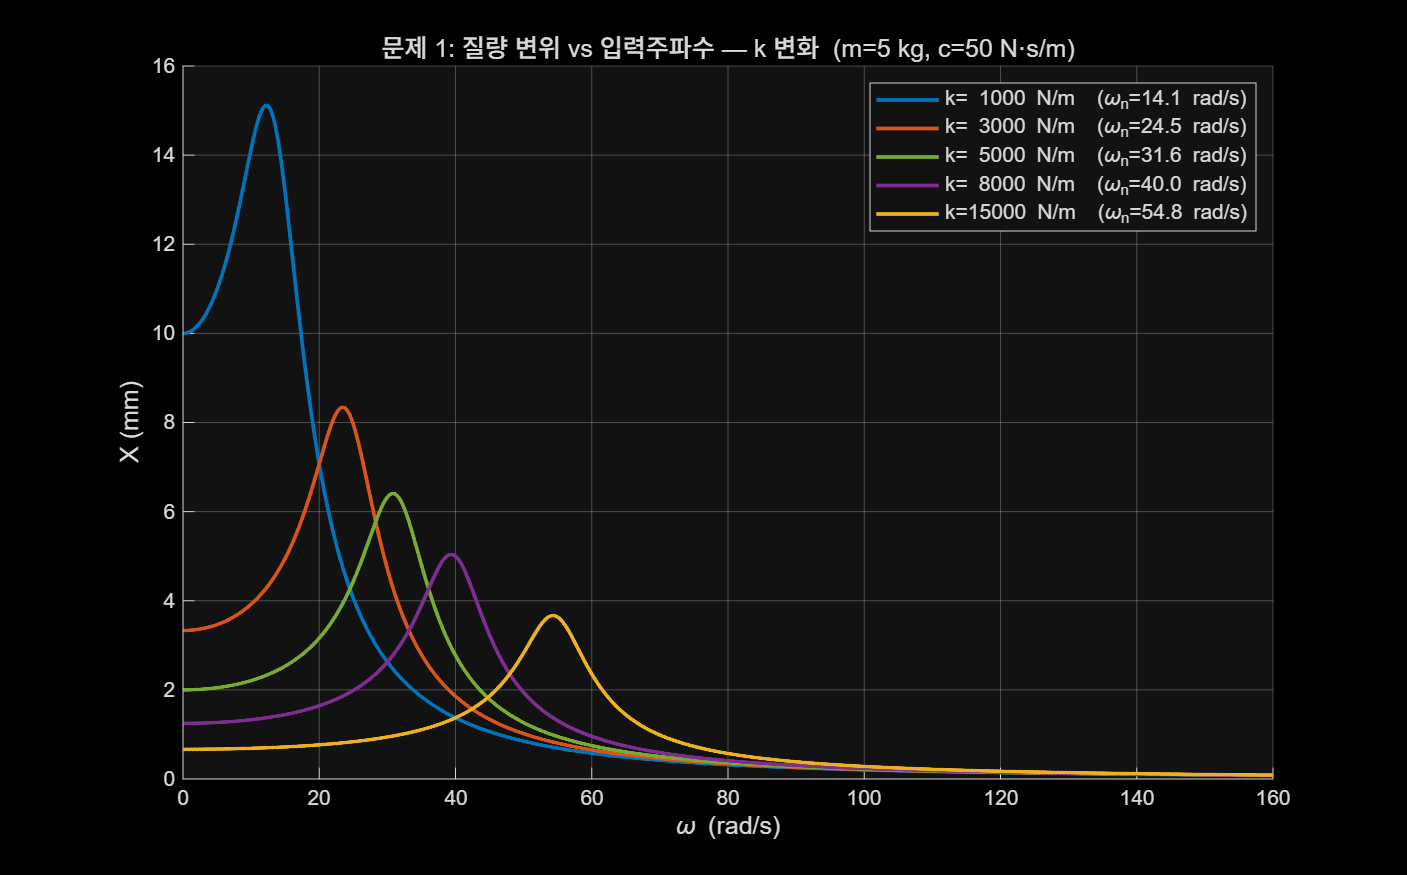
\includegraphics[width=0.80\linewidth]{figures/p1_vary_k.png}
\caption{질량 변위 vs 입력주파수 — $k$ 변화 ($m=5$, $c=50$)}
\label{fig:p1k}
\end{figure}

\begin{table}[H]
\centering
\caption{$k$ 변화에 따른 고유진동수 및 최대 변위}
\label{tab:p1k}
\begin{tabular}{rrr}
\toprule
$k$ (N/m) & $\omega_n$ (rad/s) & $X_{\max}$ (mm) \\
\midrule
1000  & 14.1 & 15.12 \\
3000  & 24.5 &  8.34 \\
5000  & 31.6 &  6.41 \\
8000  & 40.0 &  5.04 \\
15000 & 54.8 &  3.67 \\
\bottomrule
\end{tabular}
\end{table}

\begin{itemize}
  \item $k$가 커질수록 $\omega_n = \sqrt{k/m}$이 커져 공진점이 고주파 쪽으로 이동하였다.
  \item 최대 변위는 15.12 mm에서 3.67 mm로 감소하였다.
  \item 정적 변위 $F/k$도 함께 작아지므로 더 단단한 계일수록 전체 변위가 줄었다.
\end{itemize}

%% ────────────────────────────────────────────────────────────
\section{문제 2. 바닥 가진 (Base Excitation)}

\subsection{이론}

바닥 변위를 $y(t) = Y\sin(\omega t)$로 두면 운동방정식은

\begin{equation}
  m\ddot{x} + c(\dot{x} - \dot{y}) + k(x - y) = 0
\end{equation}

정리하면

\begin{equation}
  m\ddot{x} + c\dot{x} + kx = c\dot{y} + ky
\end{equation}

질량의 변위 진폭은

\begin{equation}
  X = \frac{Y\sqrt{k^2 + (c\omega)^2}}{\sqrt{(k - m\omega^2)^2 + (c\omega)^2}}
  \label{eq:p2x}
\end{equation}

전달력 진폭은 뉴턴 제2법칙($F_T = m\ddot{x}$)에 의해

\begin{equation}
  F_T = m\omega^2 X
  \label{eq:p2ft}
\end{equation}

\subsection{(a) 질량 $m$ 변화}

$c = 50$ N$\cdot$s/m, $k = 5000$ N/m 고정.

\begin{figure}[H]
\centering
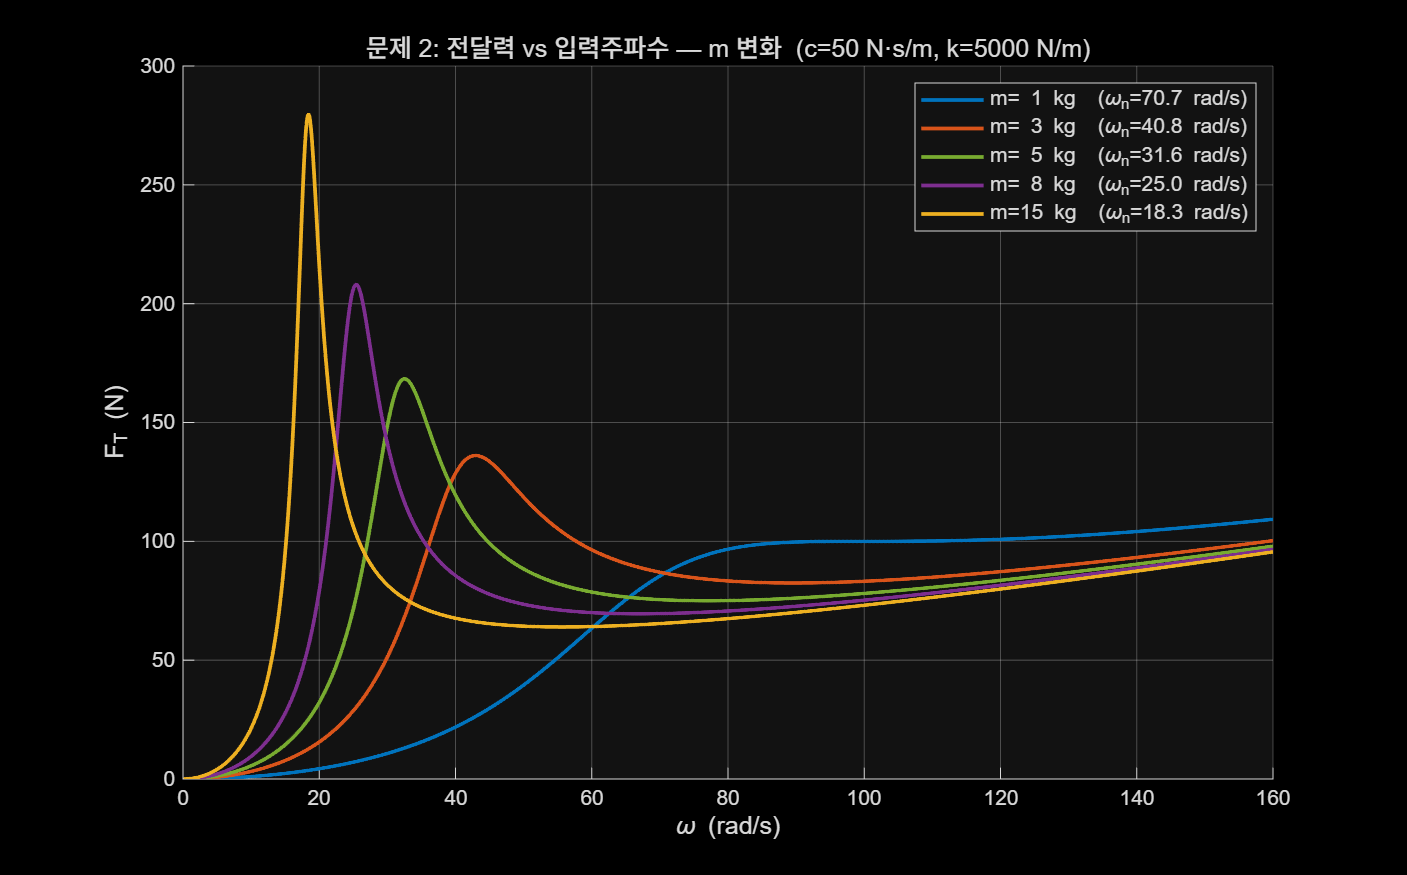
\includegraphics[width=0.80\linewidth]{figures/p2_vary_m.png}
\caption{전달력 vs 입력주파수 — $m$ 변화 ($c=50$, $k=5000$)}
\label{fig:p2m}
\end{figure}

\begin{table}[H]
\centering
\caption{$m$ 변화에 따른 최대 전달력}
\label{tab:p2m}
\begin{tabular}{rrl}
\toprule
$m$ (kg) & $F_{T,\max}$ (N) & 위치 \\
\midrule
1  & 109.3 & $\omega = 160$ (경계값) \\
3  & 136.1 & $\omega = 43.0$ (공진) \\
5  & 168.4 & $\omega = 32.5$ (공진) \\
8  & 208.0 & $\omega = 25.4$ (공진) \\
15 & 279.6 & $\omega = 18.4$ (공진) \\
\bottomrule
\end{tabular}
\end{table}

\begin{itemize}
  \item $m \geq 3$ kg에서는 질량이 커질수록 공진 전달력이 증가하였다.
  \item $m = 1$ kg은 공진 이후 고주파 증가가 더 커서 탐색 범위 끝값이 최대가 되었다.
  \item 따라서 질량의 영향은 공진 피크와 고주파 경향을 구분하여 분석해야 한다.
\end{itemize}

\subsection{(b) 감쇠 $c$ 변화}

$m = 5$ kg, $k = 5000$ N/m 고정.

\begin{figure}[H]
\centering
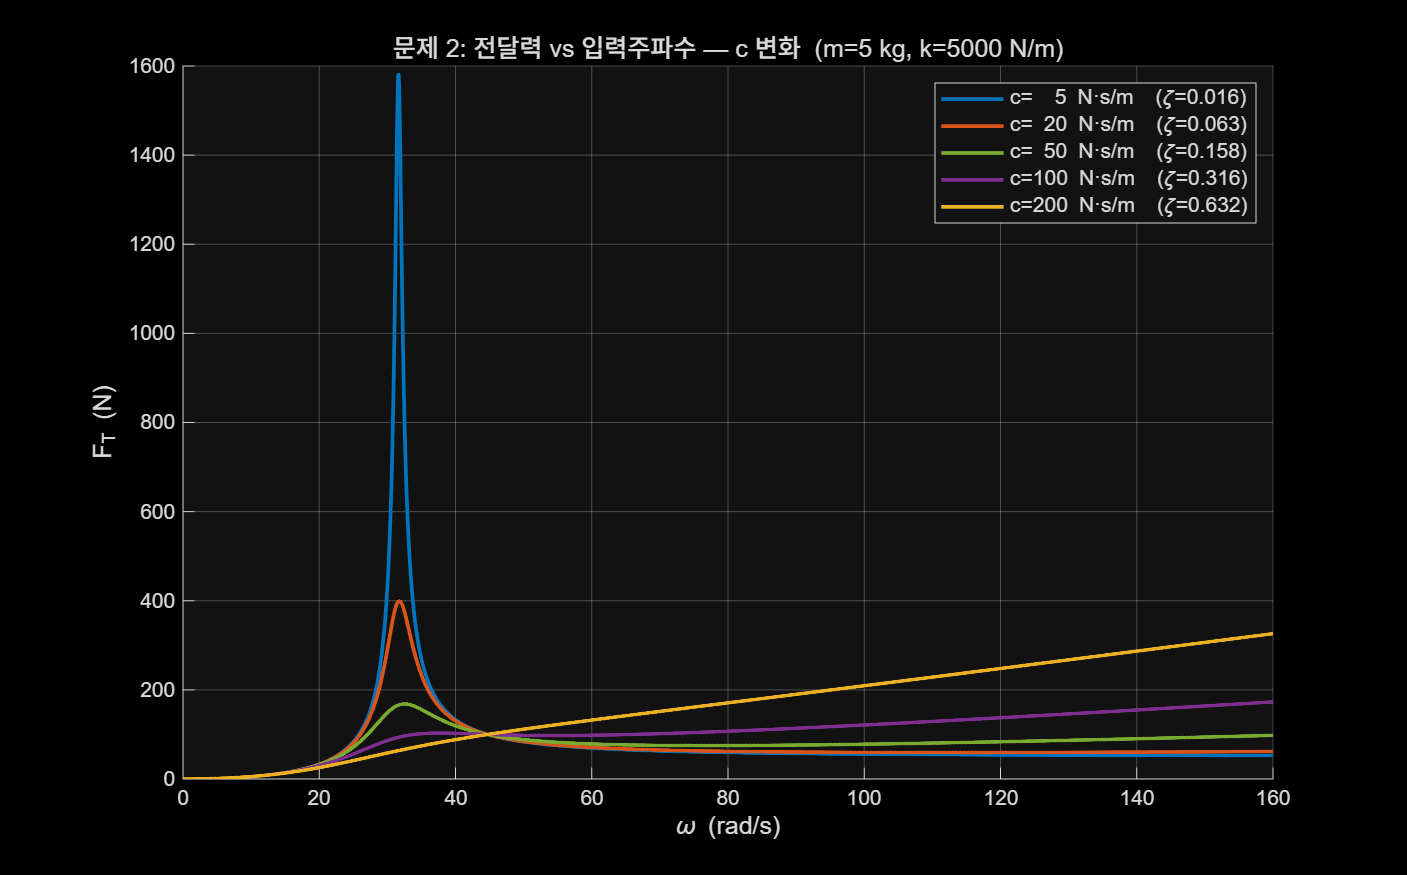
\includegraphics[width=0.80\linewidth]{figures/p2_vary_c.png}
\caption{전달력 vs 입력주파수 — $c$ 변화 ($m=5$, $k=5000$)}
\label{fig:p2c}
\end{figure}

\begin{table}[H]
\centering
\caption{$c$ 변화에 따른 최대 전달력}
\label{tab:p2c}
\begin{tabular}{rrl}
\toprule
$c$ (N$\cdot$s/m) & $F_{T,\max}$ (N) & 위치 \\
\midrule
5   & 1580.9 & $\omega = 31.6$ (공진) \\
20  &  399.2 & $\omega = 31.8$ (공진) \\
50  &  168.4 & $\omega = 32.5$ (공진) \\
100 &  173.0 & $\omega = 160$ (경계값) \\
200 &  326.2 & $\omega = 160$ (경계값) \\
\bottomrule
\end{tabular}
\end{table}

\begin{itemize}
  \item 저감쇠 구간($c \leq 50$)에서는 $c$ 증가가 공진 피크를 강하게 억제하였다.
  \item 고감쇠 구간($c \geq 100$)에서는 전달력이 공진형보다 단조 증가형으로 바뀌었다.
  \item 즉, 감쇠는 공진 억제에는 효과적이지만 고주파 전달력을 항상 줄여주지는 않는다.
\end{itemize}

\subsection{(c) 강성 $k$ 변화}

$m = 5$ kg, $c = 50$ N$\cdot$s/m 고정.

\begin{figure}[H]
\centering
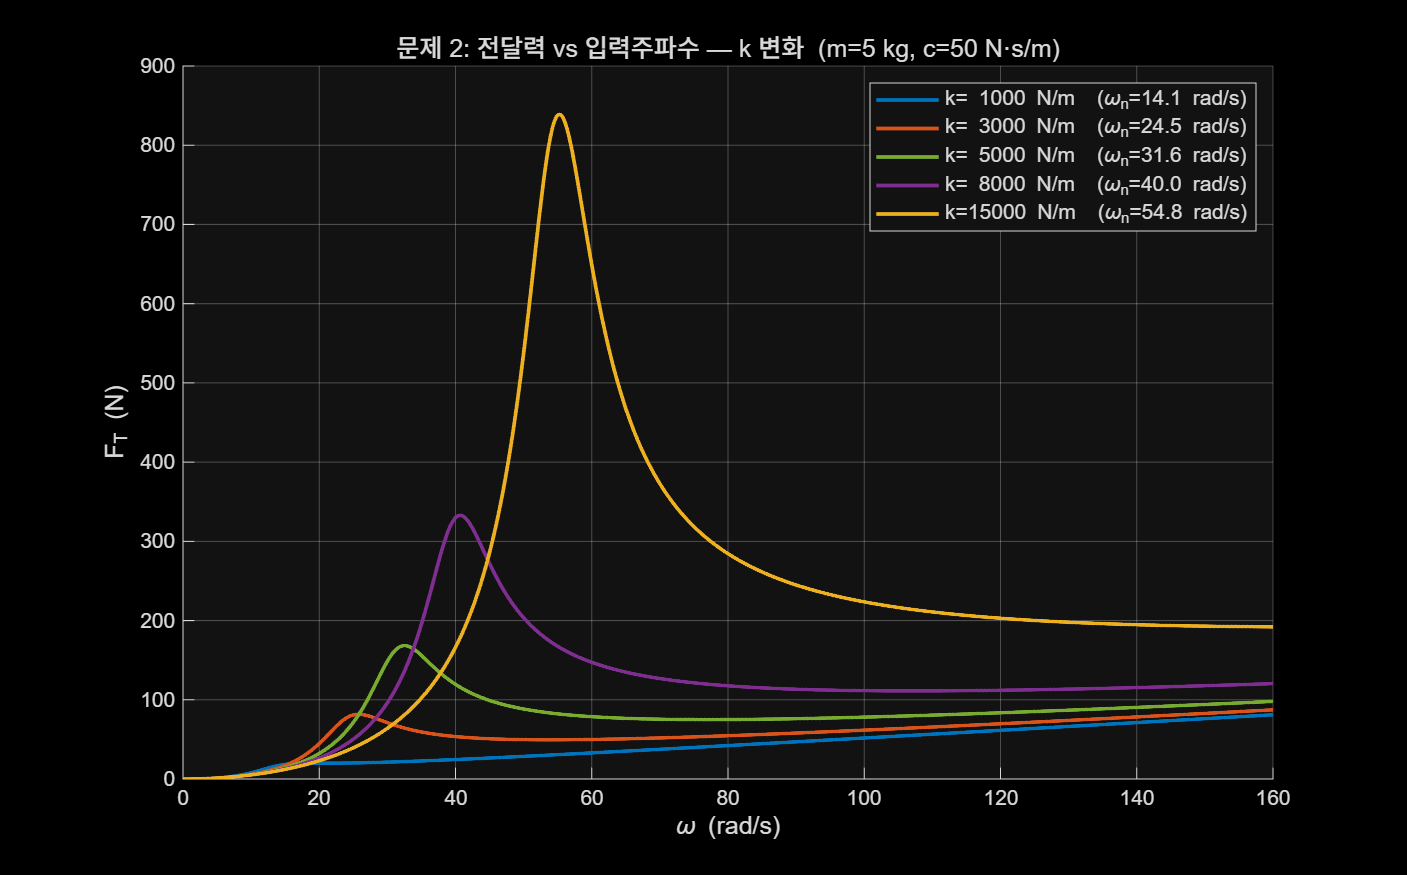
\includegraphics[width=0.80\linewidth]{figures/p2_vary_k.png}
\caption{전달력 vs 입력주파수 — $k$ 변화 ($m=5$, $c=50$)}
\label{fig:p2k}
\end{figure}

\begin{table}[H]
\centering
\caption{$k$ 변화에 따른 최대 전달력}
\label{tab:p2k}
\begin{tabular}{rrl}
\toprule
$k$ (N/m) & $F_{T,\max}$ (N) & 위치 \\
\midrule
1000  &   81.1 & $\omega = 160$ (경계값) \\
3000  &   87.3 & $\omega = 160$ (경계값) \\
5000  &  168.4 & $\omega = 32.5$ (공진) \\
8000  &  332.8 & $\omega = 40.7$ (공진) \\
15000 &  838.9 & $\omega = 55.2$ (공진) \\
\bottomrule
\end{tabular}
\end{table}

\begin{itemize}
  \item 강성이 커질수록 공진점은 고주파 쪽으로 이동하고, 공진 전달력도 크게 증가하였다.
  \item 낮은 강성에서는 공진 이후 고주파 경향으로 인해 범위 끝값이 최대가 되었다.
  \item 전달력 최소화만을 목표로 한다면 단순히 $k$를 크게 잡는 방식은 불리하다.
\end{itemize}

%% ────────────────────────────────────────────────────────────
\section{결론}

\subsection{정리}

\begin{enumerate}
  \item 조화 외력 가진에서 $c$는 공진 변위 억제에 가장 직접적인 역할을 하였다.
  \item 강성 $k$가 커지면 문제 1에서는 변위가 감소하지만, 문제 2에서는 전달력이 오히려 증가할 수 있다.
  \item 바닥 가진 문제는 공진 피크만 보면 해석이 틀릴 수 있으므로, 주파수 범위 끝값인지 함께 확인해야 한다.
\end{enumerate}

\subsection{최종 결론}

문제 1에서는 감쇠 증가가 공진 변위를 가장 효과적으로 억제하였다.
질량 증가와 강성 감소는 공진 위치를 저주파 쪽으로 이동시키며, 강성 증가는 전체 변위를 줄이는 방향으로 작용하였다.

문제 2에서는 단순히 공진 피크만 분석해서는 안 되며, 공진 이후 고주파 구간에서 전달력이 다시 커지는 경우를 함께 고려해야 한다.
특히 큰 감쇠나 작은 강성에서는 탐색 범위 상한에서 최대 전달력이 나타났으므로, 설계 목적이 공진 억제인지 고주파 전달 저감인지에 따라 해석 기준이 달라진다.

%% ────────────────────────────────────────────────────────────
\appendix
\section{MATLAB 전체 코드}

\begin{lstlisting}[caption={solve.m — 문제 1: 조화 외력 가진}]
clear; clc; close all;

F     = 10;
Y     = 0.01;
omega = linspace(0.1, 160, 3000);

clrs = [0.00 0.45 0.74;
        0.85 0.33 0.10;
        0.47 0.67 0.19;
        0.49 0.18 0.56;
        0.93 0.69 0.13];

fig_dir = fullfile(fileparts(mfilename('fullpath')), '..', 'figures');
if ~exist(fig_dir, 'dir'), mkdir(fig_dir); end

% (a) m 변화
c_f = 50;  k_f = 5000;
m_vals = [1, 3, 5, 8, 15];

fig = figure('Name','P1 Vary m', 'Position',[50 50 900 560]);
hold on;
for i = 1:length(m_vals)
    m  = m_vals(i);
    X  = F ./ sqrt((k_f - m*omega.^2).^2 + (c_f*omega).^2);
    wn = sqrt(k_f / m);
    plot(omega, X*1000, 'Color', clrs(i,:), 'LineWidth', 1.8, ...
        'DisplayName', sprintf('m=%2g kg  (\omega_n=%.1f rad/s)', m, wn));
end
xlabel('\omega (rad/s)'); ylabel('X (mm)');
legend('Location','northeast'); grid on;
saveas(fig, fullfile(fig_dir, 'p1_vary_m.png'));

% (b) c 변화
m_f = 5;  k_f = 5000;
c_vals = [5, 20, 50, 100, 200];

fig = figure('Name','P1 Vary c', 'Position',[50 50 900 560]);
hold on;
for i = 1:length(c_vals)
    c    = c_vals(i);
    X    = F ./ sqrt((k_f - m_f*omega.^2).^2 + (c*omega).^2);
    zeta = c / (2*sqrt(m_f*k_f));
    plot(omega, X*1000, 'Color', clrs(i,:), 'LineWidth', 1.8, ...
        'DisplayName', sprintf('c=%3g N·s/m  (\zeta=%.3f)', c, zeta));
end
xlabel('\omega (rad/s)'); ylabel('X (mm)');
legend('Location','northeast'); grid on;
saveas(fig, fullfile(fig_dir, 'p1_vary_c.png'));

% (c) k 변화
m_f = 5;  c_f = 50;
k_vals = [1000, 3000, 5000, 8000, 15000];

fig = figure('Name','P1 Vary k', 'Position',[50 50 900 560]);
hold on;
for i = 1:length(k_vals)
    k  = k_vals(i);
    X  = F ./ sqrt((k - m_f*omega.^2).^2 + (c_f*omega).^2);
    wn = sqrt(k / m_f);
    plot(omega, X*1000, 'Color', clrs(i,:), 'LineWidth', 1.8, ...
        'DisplayName', sprintf('k=%5g N/m  (\omega_n=%.1f rad/s)', k, wn));
end
xlabel('\omega (rad/s)'); ylabel('X (mm)');
legend('Location','northeast'); grid on;
saveas(fig, fullfile(fig_dir, 'p1_vary_k.png'));
\end{lstlisting}

\begin{lstlisting}[caption={solve.m — 문제 2: 바닥 가진}]
% (a) m 변화
c_f = 50;  k_f = 5000;

fig = figure('Name','P2 Vary m', 'Position',[50 50 900 560]);
hold on;
for i = 1:length(m_vals)
    m  = m_vals(i);
    X  = Y .* sqrt(k_f^2 + (c_f*omega).^2) ./ ...
             sqrt((k_f - m*omega.^2).^2 + (c_f*omega).^2);
    FT = m .* omega.^2 .* X;
    wn = sqrt(k_f / m);
    plot(omega, FT, 'Color', clrs(i,:), 'LineWidth', 1.8, ...
        'DisplayName', sprintf('m=%2g kg  (\omega_n=%.1f rad/s)', m, wn));
end
xlabel('\omega (rad/s)'); ylabel('F_T (N)');
legend('Location','northeast'); grid on;
saveas(fig, fullfile(fig_dir, 'p2_vary_m.png'));

% (b) c 변화
m_f = 5;  k_f = 5000;

fig = figure('Name','P2 Vary c', 'Position',[50 50 900 560]);
hold on;
for i = 1:length(c_vals)
    c    = c_vals(i);
    X    = Y .* sqrt(k_f^2 + (c*omega).^2) ./ ...
               sqrt((k_f - m_f*omega.^2).^2 + (c*omega).^2);
    FT   = m_f .* omega.^2 .* X;
    zeta = c / (2*sqrt(m_f*k_f));
    plot(omega, FT, 'Color', clrs(i,:), 'LineWidth', 1.8, ...
        'DisplayName', sprintf('c=%3g N·s/m  (\zeta=%.3f)', c, zeta));
end
xlabel('\omega (rad/s)'); ylabel('F_T (N)');
legend('Location','northeast'); grid on;
saveas(fig, fullfile(fig_dir, 'p2_vary_c.png'));

% (c) k 변화
m_f = 5;  c_f = 50;

fig = figure('Name','P2 Vary k', 'Position',[50 50 900 560]);
hold on;
for i = 1:length(k_vals)
    k  = k_vals(i);
    X  = Y .* sqrt(k^2 + (c_f*omega).^2) ./ ...
             sqrt((k - m_f*omega.^2).^2 + (c_f*omega).^2);
    FT = m_f .* omega.^2 .* X;
    wn = sqrt(k / m_f);
    plot(omega, FT, 'Color', clrs(i,:), 'LineWidth', 1.8, ...
        'DisplayName', sprintf('k=%5g N/m  (\omega_n=%.1f rad/s)', k, wn));
end
xlabel('\omega (rad/s)'); ylabel('F_T (N)');
legend('Location','northeast'); grid on;
saveas(fig, fullfile(fig_dir, 'p2_vary_k.png'));

fprintf('모든 그래프 저장 완료: %s\n', fig_dir);
\end{lstlisting}

\end{document}
